\chapter{Background}
\label{chap:bg}
In this chapter, We introduce the structure of the attack model(CNN), the method of sound signal processing(Mel-spectrogram), and the method of lifelong learning(Regularization). They are the basic of our framework.

\section{Convolutional Neural Network }


A Convolutional Neural Network (CNN) is a feed-forward neural network. Its artificial neurons can respond to a portion of the surrounding units in the coverage area and have excellent performance for large-scale image processing.

A convolutional neural network consists of one or more convolutional layers and a fully connected layer on top, and also includes associated weighting and pooling layers. This structure allows convolutional neural networks to use the two-dimensional structure of the input data. Compared to other deep learning structures, convolutional neural networks can give better results in image and speech recognition. The model can also be trained using a back propagation algorithm. Convolutional neural networks require fewer parameters to be considered than other deep feed-forward neural networks, making them an attractive deep learning structure.

\subsection{Convolutional Layers}

Each convolutional layer in a convolutional neural network consists of several convolutional units, and the parameters of each convolutional unit are optimized by a backpropagation algorithm. The purpose of the convolution operation is to extract different features of the input. The first convolutional layer may extract only some low-level features such as edges, lines, and corners. More layers of the network can iteratively extract more complex features from the low-level features. For example, using a 3x3 convolution kernel requires only 9 learnable parameters since each region has the same shared weights, regardless of the size of the input image. Using regular weights on fewer parameters avoids the gradient disappearance and gradient explosion problems that can occur during backpropagation.

\begin{figure}[H]
	\centering
	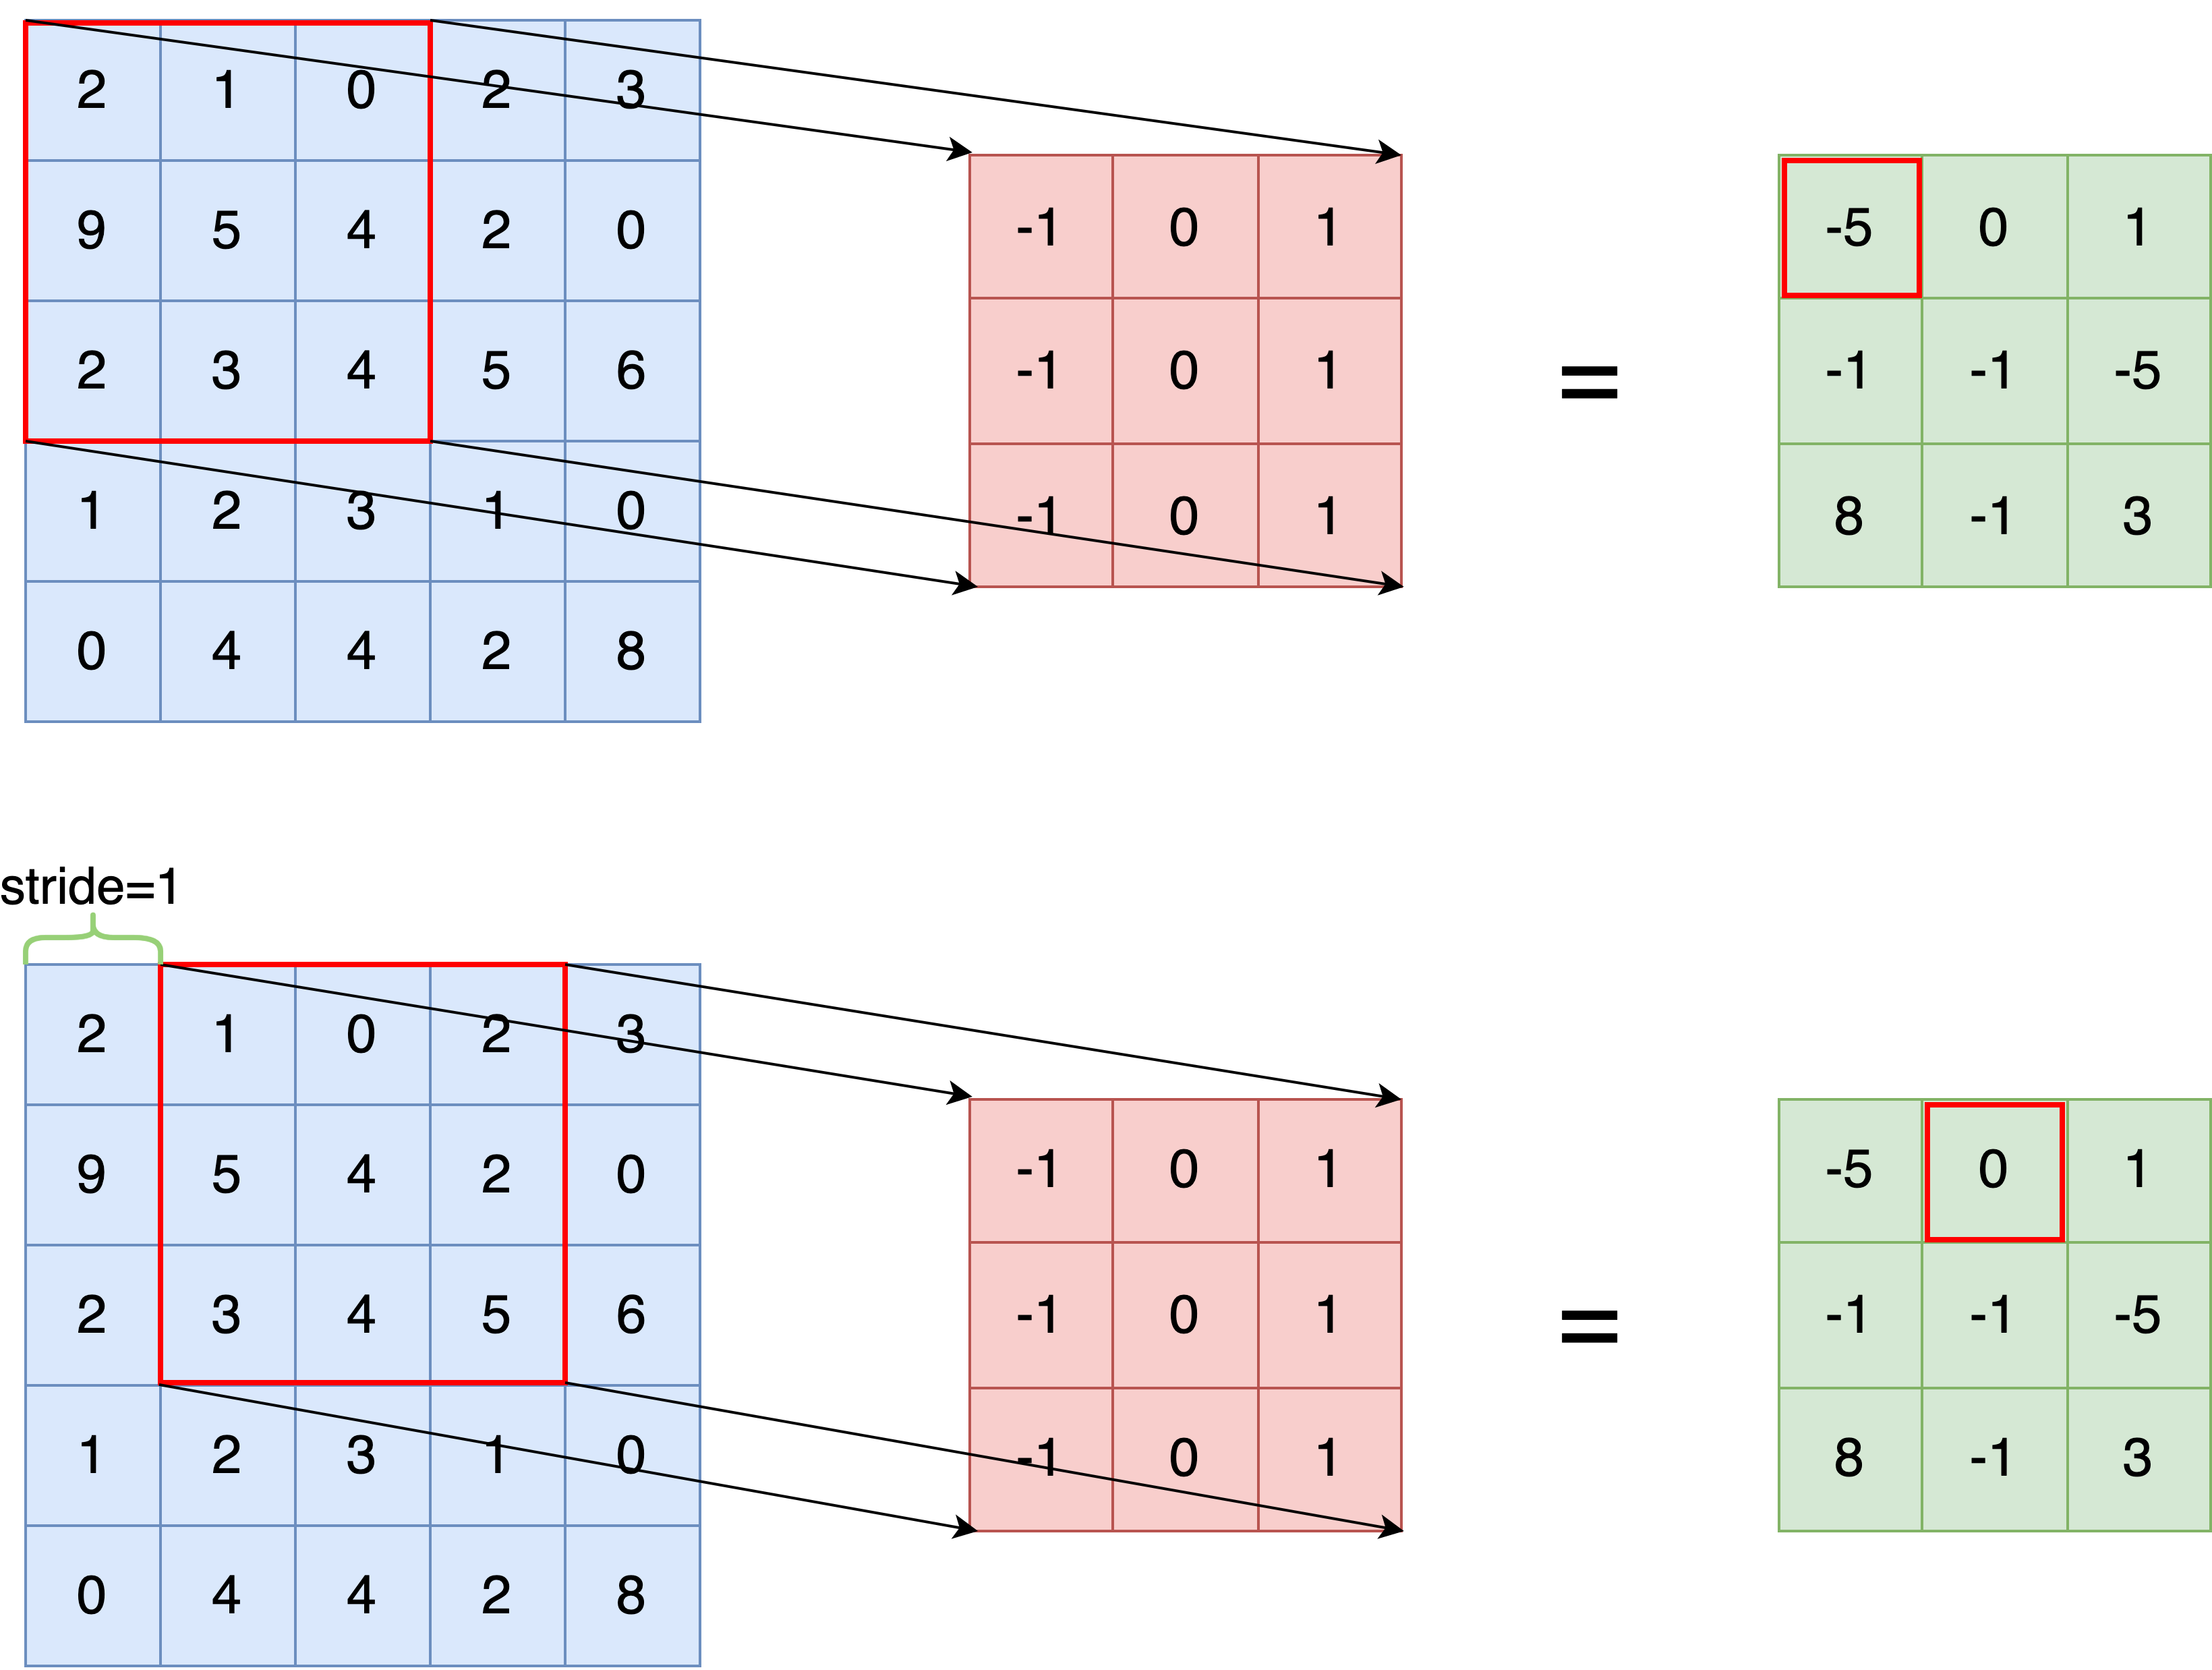
\includegraphics[width=0.6\linewidth]{figures/conv}
	\caption[An example of two-dimensional convolution]{A simple two dimensional convolution with a 3x3 convolutional kernel and stride = 1, the output size is 3x3 which is decided by image size, kernel size and stride.}
	\label{fig:conv}
\end{figure}

\subsection{Pooling Layers}

Pooling is also important concept in convolutional neural networks, and it is actually a form of downsampling. There are many different forms of nonlinear pooling functions, of which maximum pooling (see Figure ~\ref{fig:maxpool} for an example) is the most common. It divides the input image into several rectangular regions and outputs the maximum value of each subregion. Intuitively, this mechanism works because after a feature is found, its exact position is much less important than its relative position to other features. The pooling layer continuously reduces the size of the data space, so the number of parameters and the amount of computation are also reduced, which also controls overfitting to some extent. Usually, the pooling layer is inserted periodically between the convolutional layers of the CNN.

\begin{figure}[H]
	\centering
	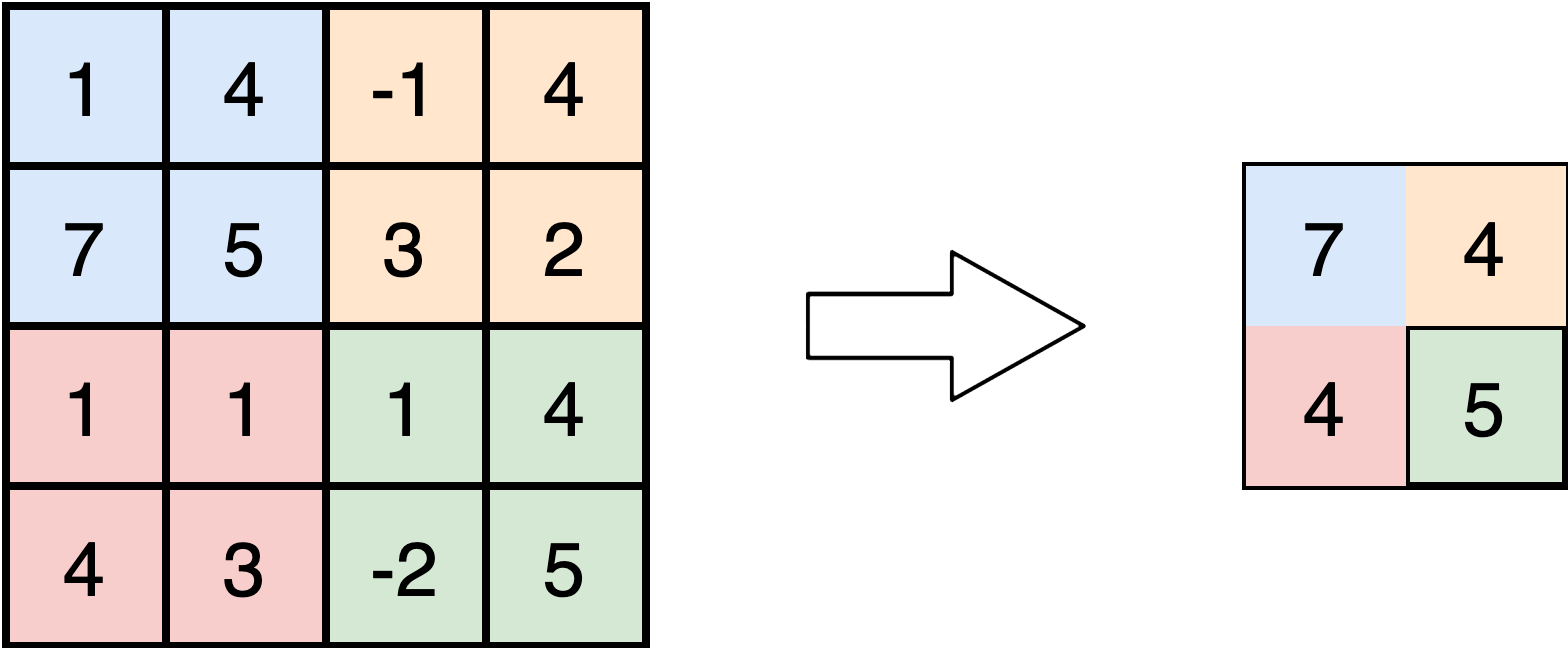
\includegraphics[width=0.6\linewidth]{figures/maxpool}
	\caption[An example of max pooling]{An example of max pooling with a 2x2 kernel and the stride is 2.}
	\label{fig:maxpool}
\end{figure}

\subsection{Fully Connection Layers}

In a CNN structure, one or more fully connected layers are connected after multiple convolutional and pooling layers. Similar to a multilayer perceptron (MLP), each neuron in a fully connected layer is fully connected to all neurons in the previous layer. The fully connected layers can combine local information with category differentiation in the convolutional or pooling layers. To improve the performance of the CNN network, the activation function of each neuron in the fully connected layer generally uses the ReLU function. The output value of the last fully connected layer is passed to an output that can be classified by softmax regression. This layer can also be referred to as a softmax layer. For a specific classification task, it is important to choose the appropriate loss function. CNNs have several commonly used loss functions, each with different characteristics. Generally the fully connected layer of CNN has the same structure as MLP, and the training algorithm of CNN mostly uses BP algorithm.
\begin{figure}[H]
	\centering
	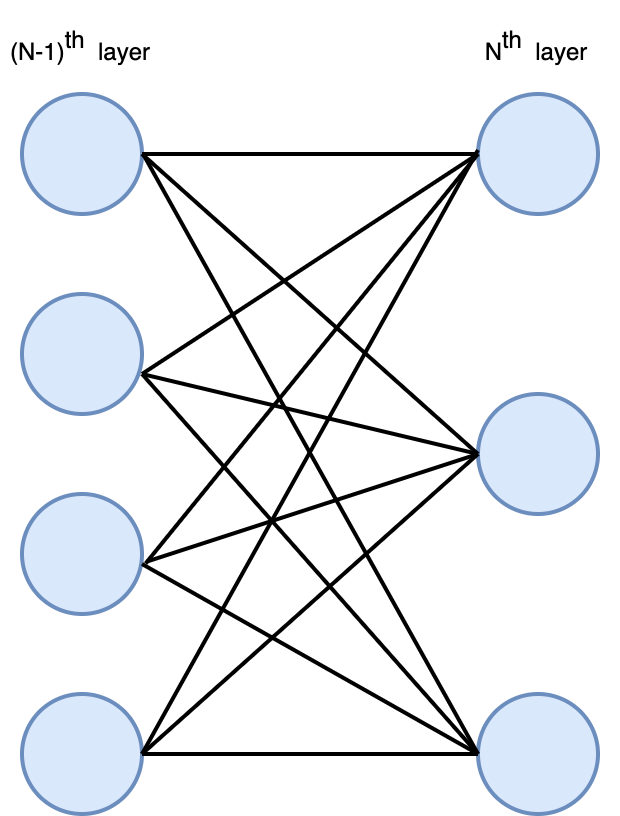
\includegraphics[width=0.4\linewidth]{figures/fc}
	\caption[The structure of fully connection layer]{The structure of fully connection layer.}
	\label{fig:fclayer}
\end{figure}


\section{Regularization Method}
\label{section:transformer}
Regularization is a general term for a class of methods in machine learning that introduce additional information to the original loss function in order to prevent overfitting and improve model generalization performance. That is, the objective function becomes the $original loss function + extra items$. There are generally two kinds of commonly used extra items, which are called $\ell 1-n o r m$ and $\ell 2-n o r m$.

\subsection{Regularized Formula}

$L1$ regularization and $L2$ regularization can be seen as penalty terms of the loss function. By penalty, we mean some restrictions on certain parameters in the loss function. For linear regression models, a model using $L1$ regularization is called Lasso regression and a model using $L2$ regularization is called Ridge regression.

Linear regression $L1-regularized$ loss function:
$$
\min _{w}\left[\sum_{i=1}^{N}\left(w^{T} x_{i}-y_{i}\right)^{2}+\lambda\|w\|_{1}\right]
$$

$L1 regularization$ is the sum of the absolute values of each element in the weight vector $w$, which is usually expressed as $\|w\|_{1}$.

Linear regression $L2-regularized$ loss function:
$$
\min _{w}\left[\sum_{i=1}^{N}\left(w^{T} x_{i}-y_{i}\right)^{2}+\lambda\|w\|_{2}^{2}\right]
$$
The $L2 regularization$ is the sum of the squares of the elements in the weight vector $w$ and then the square root (you can see that the $L2 regularization$ term of the Ridge regression has the square symbol), which is usually expressed as $\|w\|_{2}^{2}$.

A coefficient$\lambda$, denoted by $\alpha$ in Python, is usually added before the regularization term, and this coefficient is the hyperparameter to be tuned.

\subsection{Role Of Regularization}
L1 regularization can make the parameters sparse, i.e., the parameters obtained are a sparse matrix that can be used for feature selection.
\begin{itemize}
	\item \textbf{Sparsity.}It means that many parameters of the model are 0. Usually the number of features in machine learning is large, for example, in text processing, if a term is used as a feature, the number of features can reach tens of thousands (bigram). In prediction or classification, it is obviously difficult to select so many features, but if the model obtained by substituting these features is a sparse model, many parameters are 0, which means that only a few features contribute to the model, and most of the features do not contribute, and even if they are removed, they have no effect on the model, so we can only focus on the features with non-zero coefficients. This is equivalent to a feature selection of the model, leaving only some more important features to improve the generalization ability of the model and reduce the possibility of overfitting.
\end{itemize}

$L2 regularization$ prevents model overfitting; to some extent, $L1-norm$ also prevents overfitting.

\subsection{L1 Regularization And Sparsity}

In $L1 regularization$, in order to constrain the space of possible values of $w$ and thus prevent overfitting, we add a constraint to this optimization problem that the $L1 parametrization$ of $w$ cannot be greater than $m$.
$$
\left\{\begin{array}{l}
	\min \sum_{i=1}^{N}\left(w^{T} x_{i}-y_{i}\right)^{2} \\
	s . t .\|w\|_{1} \leqslant m
\end{array}\right.
$$
The problem is transformed into a convex optimization problem with constraints and the Lagrangian function is written:
$$
\sum_{i=1}^{N}\left(w^{T} x_{i}-y_{i}\right)^{2}+\lambda\left(\|w\|_{1}-m\right)
$$

Let $W_{*}$  and $\lambda_{*}$ be optimal solutions of the original problem, then by the KKT condition we have:
$$
\left\{\begin{array}{l}
	0=\nabla_{w}\left[\sum_{i=1}^{N}\left(W_{*}^{T} x_{i}-y_{i}\right)^{2}+\lambda_{*}\left(\|w\|_{1}-m\right)\right] \\
	0 \leqslant \lambda_{*}
\end{array}\right.
$$
Let the L1 regularized loss function: $
J=J_{0}+\lambda \sum_{w}|w|$,where$J_{0}=\sum_{i=1}^{N}\left(w^{T} x_{i}-y_{i}\right)^{2}$is the original loss function, the term after the plus sign is the $L1 regularization$ term, and $\lambda$ is the regularization factor.
Notice that the $L1 regularization$ is the sum of the absolute values of the weights and $J$ is a function with absolute value sign, so $J$ is not completely differentiable. The task of machine learning is to find the minimum of the loss function by some method (e.g. gradient descent). When we add the $L1 regularization$ term after the original loss function $J_{0}$, it is equivalent to putting a constraint on $J_{0}$. Let $
L=\lambda \sum_{w}|w|$,then $J=J_{0}+L
$, at which point our task becomes to find the solution under the $L$ constraint where $J_{0}$ takes the minimum value.

Consider the two-dimensional case, i.e., there are only two weights $w1$ and $w2$, when $L=\left|w_{1}\right|+\left|w_{2}\right|$For the gradient descent method, the process of solving $J_{0}$ can be drawn as an equivalence line, while the $L_{1}$ regularized function $L$ can also be drawn in the two-dimensional plane of $w_{1}$ and $w_{2}$. The following figure:
\begin{figure}[!htbp]
	\centering
	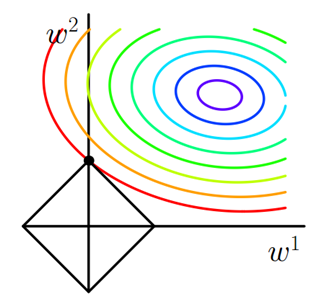
\includegraphics[width = 0.7\textwidth]{figures_ning/l1.png}
	\caption[The architecture of Faster R-CNN]
	{ L1 Regularization.}
	\label{fig:l1}
\end{figure}

The contour in the figure above is the contour of $J_{0}$ and the black square is the graph of the $L$ function. In the figure, the optimal solution is found when the $J_{0}$ contour intersects the graph of $L$ for the first time. In the above graph $J_{0}$ and $L$ intersect at a vertex of $L$. This vertex is the optimal solution. Notice that the value of this vertex is $\left(w_{1}, w_{2}\right)=\left(0, w_{2}\right)$. It can be intuitively imagined that because the $L$ function has many prominent corners (four in the two-dimensional case and more in the multidimensional case), the chance of $J_{0}$ coming into contact with these corners will be much greater than the chance of coming into contact with the rest of $L$. At these corners, there will be many weights equal to zero, which is why $L_{1} regularization$ can produce a sparse model, which in turn can be used for feature selection.

The coefficient $\lambda$ in front of the regularization can control the size of the graph of $L$. The smaller $\lambda$ is, the larger the graph of $L$ (the black box in the above figure); the larger $\lambda$ is, the smaller the graph of $L$ can be so small that the black box is only a little beyond the origin range, which is the most advantageous value  $\left(w_{1}, w_{2}\right)=\left(0, w_{2}\right)$ in which $w_{2}$ can be taken to a very small value.

Similarly, and $L_{2}$ regularized loss function: $J=J_{0}+\lambda \sum_{w} w^{2}$,the same can be drawn its image in the two-dimensional plane as follows:
\begin{figure}[!htbp]
	\centering
	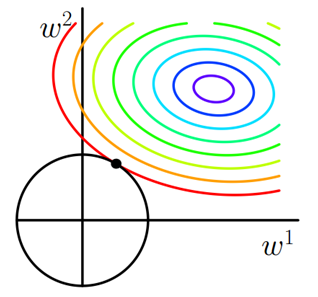
\includegraphics[width = 0.7\textwidth]{figures_ning/l2.png}
	\caption[L2 Regularization]
	{ L2 Regularization.}
	\label{fig:l2}
\end{figure}

The graph of the $L_{2}-regularized$ function in the two-dimensional plane is a circle, which is ground away from the corners compared to a square. Therefore the chance of making $w_{1}$ or $w_{2}$ equal to zero when $J_{0}$ intersects $L$ is much smaller, which is why the $L_{2}-regularization$ is not sparse

\subsection{$\ell 1-n o r m$ Prevents Overfitting}

The fitting process usually tends to make the weights as small as possible and finally construct a model with all parameters relatively small. This is because it is generally believed that models with small parameter values are simpler, can be adapted to different data sets, and also avoid the overfitting phenomenon to some extent. For a linear regression equation, if the parameters are large, then as long as the data is shifted a little, it will have a great impact on the results; but if the parameters are small enough, a little more data shift will not have any impact on the results, that is, it is highly resistant to perturbation.

Take the gradient descent method in linear regression as an example. Assuming that the required parameter is $\theta$ and  $h \theta(x)$ is our assumed function, the cost function of linear regression is as follows:
$$
J_{\theta}=\frac{1}{2 n} \sum_{i=1}^{n}\left(h \theta\left(x^{(i)}\right)-y^{(i)}\right)^{2}
$$
The iterative formula for $\theta$ in gradient descent is:
$$
\theta_{j}=\theta_{j}-\alpha \frac{1}{n} \sum_{i=1}^{n}\left(h \theta\left(x^{(i)}\right)-y^{(i)}\right) x_{j}^{(i)}
$$

where $\alpha$ is the learning rate. The above equation is the iterative formula without adding the $L_{2}$ regularization term. If $L_{2}$ regularization is added after the original cost function, the iterative formula is:
$$
\theta_{j}=\theta_{j}\left(1-\alpha \frac{\lambda}{n}\right)-\alpha \frac{1}{n} \sum_{i=1}^{n}\left(h \theta\left(x^{(i)}\right)-y^{(i)}\right) x_{j}^{(i)}
$$

where $\lambda$ is the regularization parameter. As can be seen from the above equation, compared to the iterative formula without adding $L2 regularization$, at each iteration, $\theta_{j}$ is first multiplied by a factor less than 1, which makes $\theta_{j}$ decreasing, so in total, $\theta$ is decreasing.Therefore $L2$ regularization can obtain smaller parameters and thus prevent overfitting.

\section{Signal Processing}

The first step of machine learning is to extract the corresponding features. If the input data is a picture, for example, a 28*28 picture, then only each pixel needs to be used as a feature, and the corresponding pixel value size (representing the intensity of the color) can be used as the feature value. Then in the field of audio and speech signal processing, we need to convert the signal into a corresponding speech spectrogram, and use the data on the speech spectrogram as the features of the signal. The horizontal axis $x$ of the spectrogram is time, the vertical axis $y$ is frequency, and the value corresponding to $(\mathrm{x}, \mathrm{y})$ represents the amplitude of frequency $y$ at time $x$. However, the human ear is logarithmic in its perception of frequency, i.e., sensitive to changes in the lower frequency bands and sluggish to changes in the higher frequency bands, so a linearly distributed speech spectrogram is obviously "not useful enough" for feature extraction, so the Meier speech spectrogram Therefore, the Meier spectrum map was created. The vertical frequency and the original frequency of Meier's speech spectrogram are interchanged by the following formula:
$$
\begin{gathered}
	m=2595 \log _{10}\left(1+\frac{f}{700}\right) \\
	f=700\left(10^{m / 2595}-1\right)
\end{gathered}
$$

$f$ represents the original frequency and $m$ represents the transformed Mel frequency. Obviously, when $f$ is large, the change of m tends to be flat. And the Meier cepstrum coefficients (MFCCs) are obtained by cosine transformation (DCT, a linear transformation similar to the Fourier transform) and then taking some of the coefficients.
The Melody score chart is divided into the following steps. An audio file is used as an example to show the principle of each step.

\subsection{Get Audio Signal}

python can use the librosa library to read audio files, but for MP3 files, it will automatically call the audio read function, so if it is an MP3 file, make sure to add the path to ffmpeg.exe to the system environment variable, otherwise the audio read function will error out. Here we first read the audio file and make a waveform from 0-20 seconds. Nowadays, the sampling rate of music files is usually 44.1 kHz. 
\begin{figure}[!htbp]
	\centering
	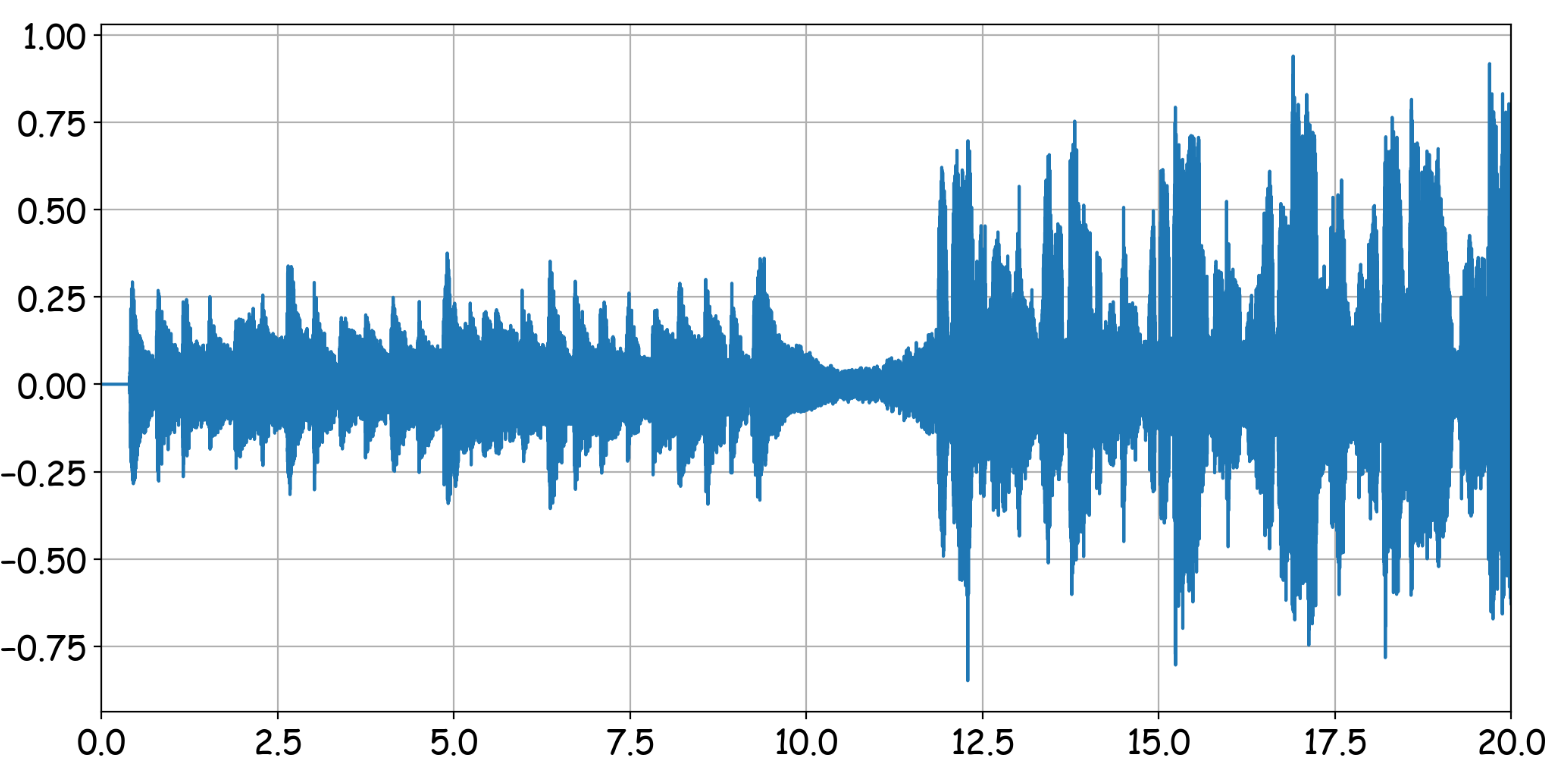
\includegraphics[width = 0.7\textwidth]{figures_ning/audio_1.png}
	\caption[L2 Regularization]
	{ Amplitude of audio signal.}
	\label{fig:audio_1}
\end{figure}

\subsection{Pre-Emphasis}

Generally speaking, the high-frequency component of the speech/audio signal has a small strength and the low-frequency component has a large strength. Signal pre-emphasis is to let the signal pass through a high-pass filter so that the strengths of the high and low frequency components of the signal do not differ too much. In the time domain, the signal $x[n]$ is operated as follows:
$$
y[n]=x[n]-\alpha x[n-1]
$$

$\alpha$ is usually taken as a value very close to 1, with a typical value of 0.97 or 0.95. From the time domain formula, some people may not understand why this is a high-pass filter, so let's look at the transfer function of the filter from the perspective of z-transform:
$$
H(z)=\frac{Y(z)}{X(z)}=1-\alpha z^{-1}=\frac{z-\alpha}{z}
$$

It can be seen that the filter has a pole 0 and a zero point $\alpha$. When the frequency is 0, z=1, the amplification factor is $(1-\alpha)$. As the frequency increases, the amplification factor becomes larger, and when the frequency reaches $p_{i}$, the amplification factor is $(1+ \alpha)$. In the discrete domain, $[0, p_{i}]$ corresponds to $[0, \mathrm{fs} / 2]$ in the continuous domain (in Hz). Where fs is the sampling rate, which in our case is 44.1 kHz. so the amplification factor is $(1+ \alpha)$ when the frequency goes to 22000 Hz. The following figure shows the generated graph:
\begin{figure}[!htbp]
	\centering
	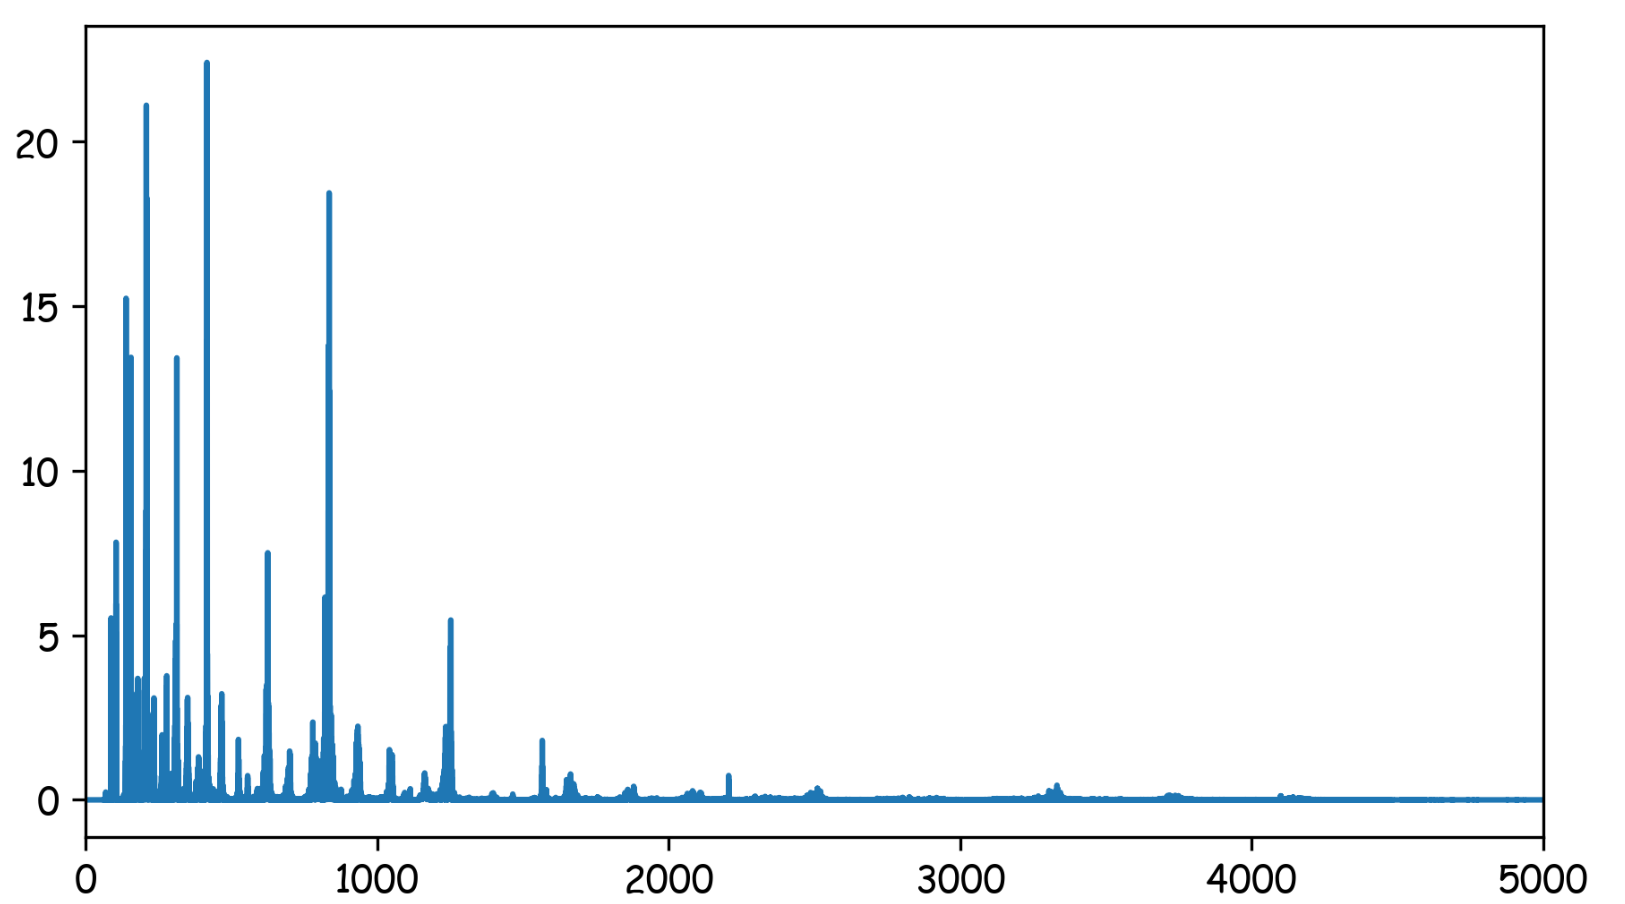
\includegraphics[width = 0.7\textwidth]{figures_ning/audio_2.png}
	\caption[Unpre-emphasized signal spectrum]
	{ Unpre-emphasized signal spectrum}
	\label{fig:audio_2}
\end{figure}

\begin{figure}[!htbp]
	\centering
	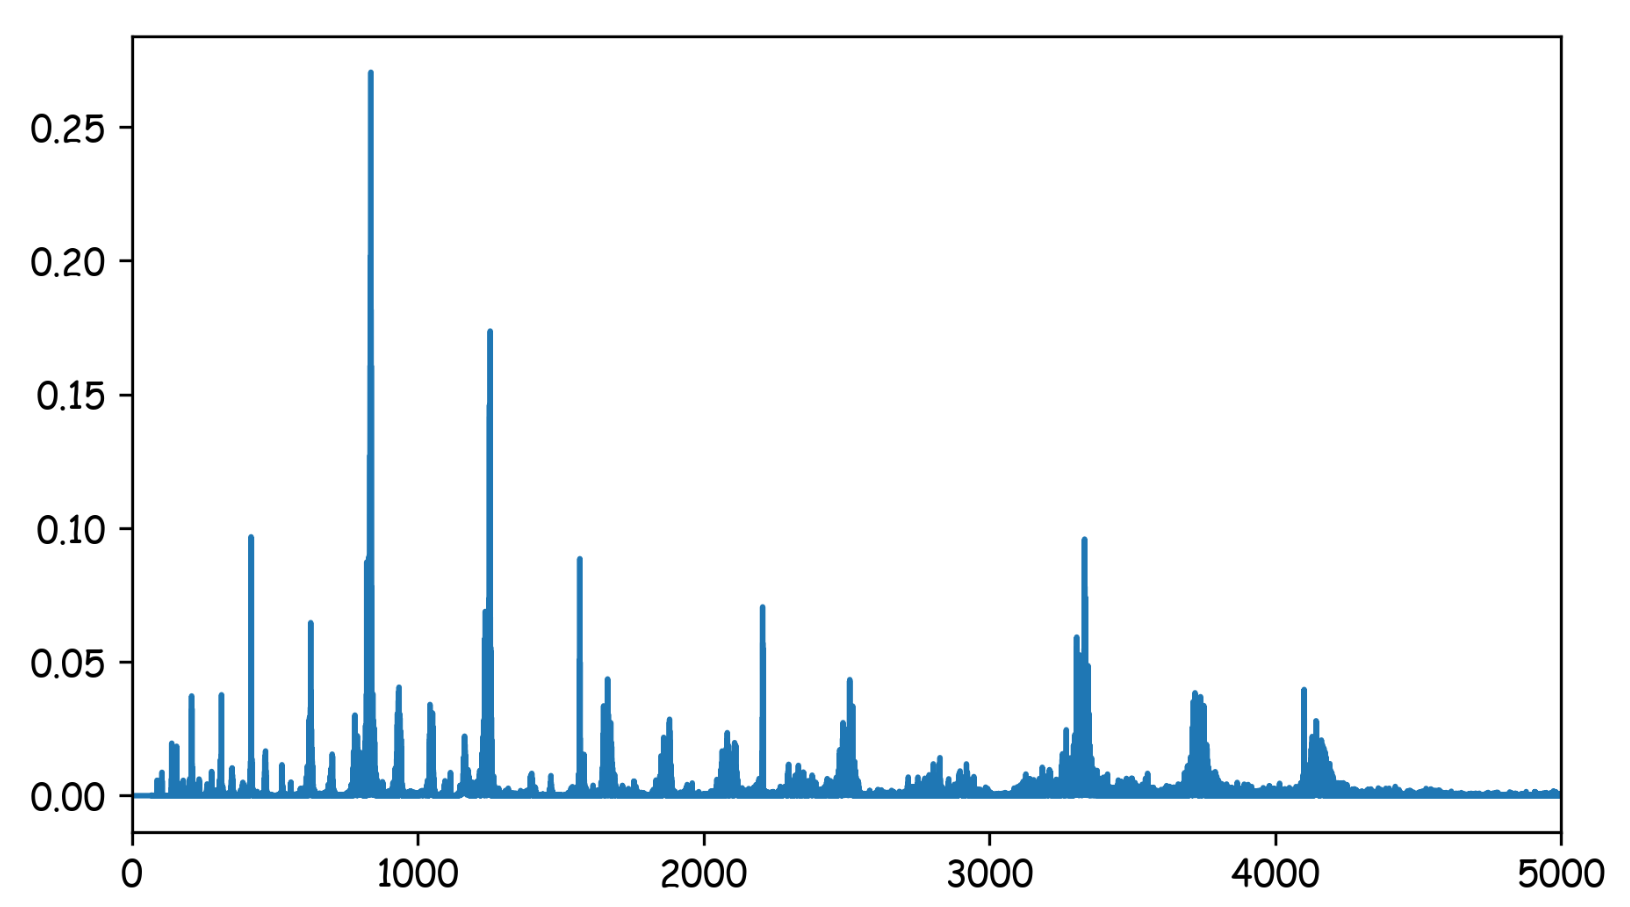
\includegraphics[width = 0.7\textwidth]{figures_ning/audio_3.png}
	\caption[Pre-emphasized signal spectrum]
	{ Pre-emphasized signal spectrum}
	\label{fig:audio_3}
\end{figure}

The code of both graphs uses the function librosa.fft.rfft(y,n), $rfft$ means that after the FFT transform only half of it is taken (because the other half corresponds to negative frequencies, which are useless), $y$ corresponds to the signal, and $n$ corresponds to the number of points to do the FFT. The actual frequency corresponding to each point is the index value of the point ${ }^{*} \mathrm{f_{s}} / \mathrm{n}$. How is this obtained? Because the 882,000th point should correspond to (approximately equal to) $f_{s}$ (or 2$p_{i}$ in the discrete domain), so the previous points can correspond one by one according to the linear relationship. Only 0-5000Hz is shown here, and it can be seen that the difference between the high-frequency component of the signal after pre-emphasis and the low-frequency component is obviously not so big.
The result of pre-emphasis:
\begin{enumerate}[\qquad  1.]
	\item Balance between high and low frequencies.
	\item Avoid numerical problems in the FFT (i.e., high frequency values that appear too small in the denominator may go wrong).
	\item Possible improvement of SNR.
\end{enumerate}

\subsection{Framing}

The time covered by the original signal is too long, and using it as a whole to do FFT, we can only get the relationship between signal frequency and intensity, and lose the time information. Therefore, after pre-processing the signal, the original signal should be divided into several small pieces according to time, and one piece is called a frame. We want to get the relationship between frequency and time, so we divide the original signal into several frames, make FFT for each frame (also called short-time FFT, because we only take a small period of time), and then stitch the obtained results together in time order. This is the principle of spectrogram.
Several variables are defined below:
\begin{itemize}
	\item \textbf{Frame Size:} Length of each frame. Usually it is 20-40ms, too long will result in a small time resolution, too small will increase the computational cost. Here we take 25ms.
	\item \textbf{Frame Length:} The number of samples per frame. This is equal to ${ }^{*} f_{s}*frame_size$, which is 44.1k*0.025=1102.
	\item \textbf{Frame Stride:} The interval between two adjacent frames. Usually the interval must be less than the length of each frame, i.e. there should be an overlap between the two frames, otherwise the information near the boundary of the two frames may be removed. When doing feature extraction, it is never desirable to remove the useful information. Here we take 10ms, i.e. there is $60 \%$overlap.
	\item \textbf{Frame Step:} The number of samples in two adjacent frames. Here is 441.
	\item \textbf{Frame Num:} The number of frames needed for the entire signal. The number of frames needed is generally expected to be an integer value, so the signal should be zero padded so that the length of the signal can be divided into integer frames.
\end{itemize}

\subsection{Window}

After splitting the frames, a window function is added to each frame to get a better sidelobes. Usually a hamming window is used.

In this process of frame splitting, it is equivalent to adding a rectangular window to the signal, the spectrum of the rectangular window has a large sidelobes, and the window function is multiplied with the original function in the time domain, which is equivalent to the convolution in the frequency domain. This is the spectral leakage.

\subsection{Power Spectrum}

Since each line is a 1102-point signal, we can choose a 1024-point FFT (fewer FFT points than the original signal will reduce the frequency resolution, but the difference here is small, so we can (ignore). The power spectrum is obtained by taking the magnitude of the obtained FFT transform and dividing it by the corresponding number of FFT points. At this point we have actually obtained the spectrogram, we just need to use plt.imshow to draw the heat map corresponding to its dB value.
\begin{figure}[!htbp]
	\centering
	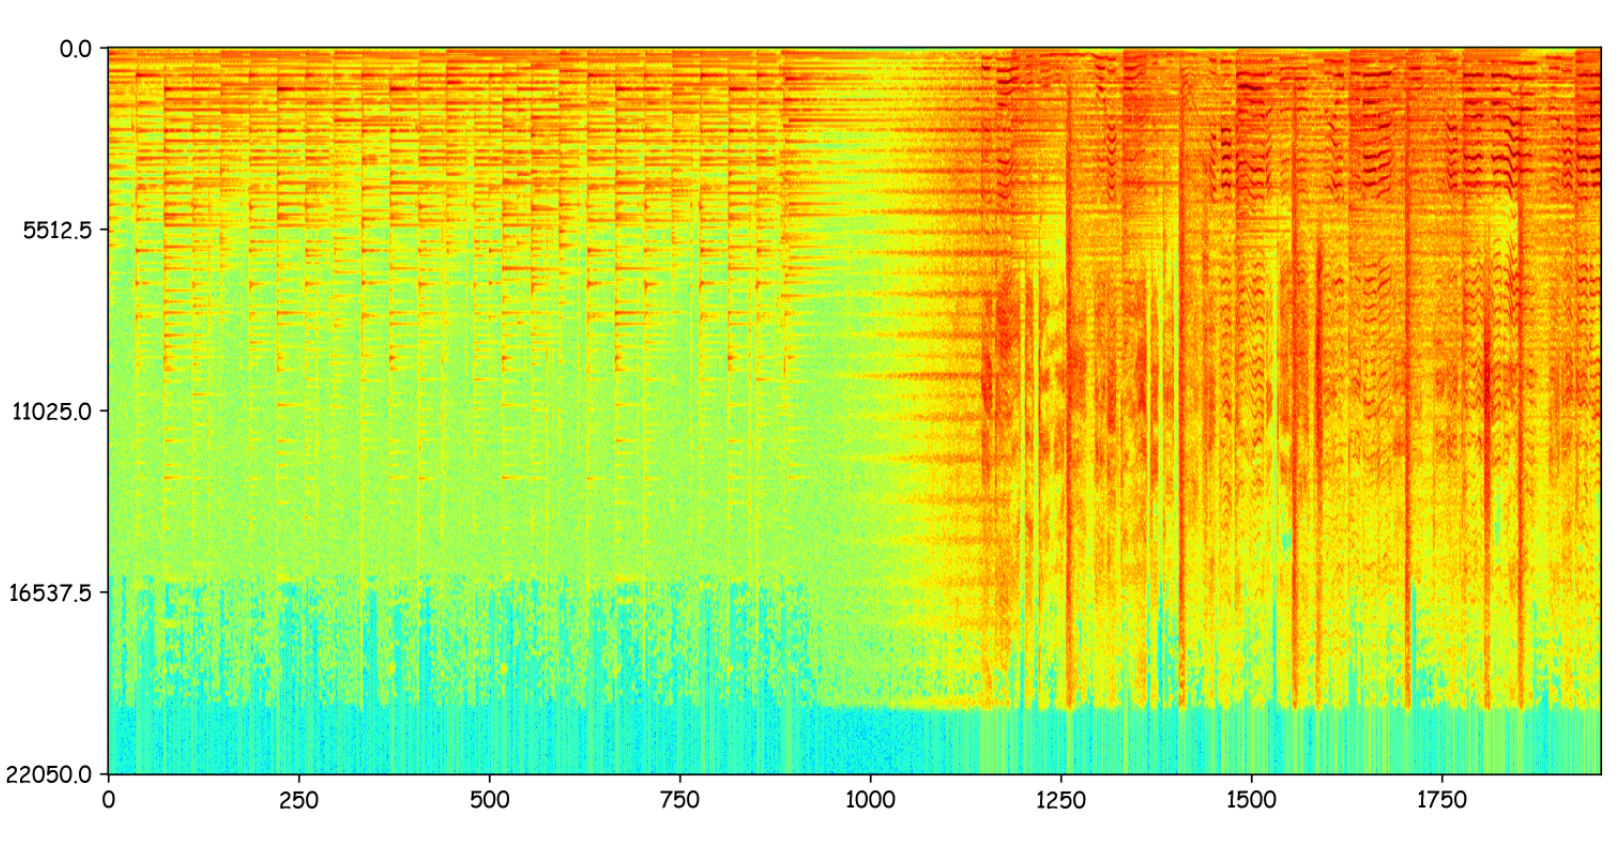
\includegraphics[width = 0.7\textwidth]{figures_ning/audio_4.png}
	\caption[Heat Map]
	{ Heat Map}
	\label{fig:audio_4}
\end{figure}

\subsection{Mel-filter Banks}

The last step is to apply the Mel filter to the pow-frames obtained in the previous step. The so-called Mayer filter bank is a triangular filter bank of equal height, where each filter starts at the midpoint of the previous filter. The corresponding frequencies are linear on the Meier scale, hence the name Meier filter bank. The frequency corresponding to each filter can be converted from the maximum frequency (4000 in the figure below, 22.05k in our case) to the Mel frequency using the formula mentioned above, divided linearly into several frequency bands on the Mel scale, and then converted back to the actual frequency scale. In practice, each filter is dotted with the power spectrum pow-frames and the result is the energy in the band. Here our pow-frames is a (1999,513) matrix, Mel filter fbank is a (mel-N, 513) matrix, where mel-N represents the number of corresponding Mel filters, this value can not be too large, because here we only have a total of 513 points, if mel-N is too large, will lead to the length of the first few filters are If mel-N is too large, the length of the previous filters will be 0 (because the low-frequency mel filters are particularly narrow). T can be obtained by multiplying these two matrices by pow-frames*F-bank.T. The result is a (1999, 40) matrix, where each row is a frame and each column represents the energy of the corresponding mel band. An example of a specific mel filter is shown below:
\begin{figure}[!htbp]
	\centering
	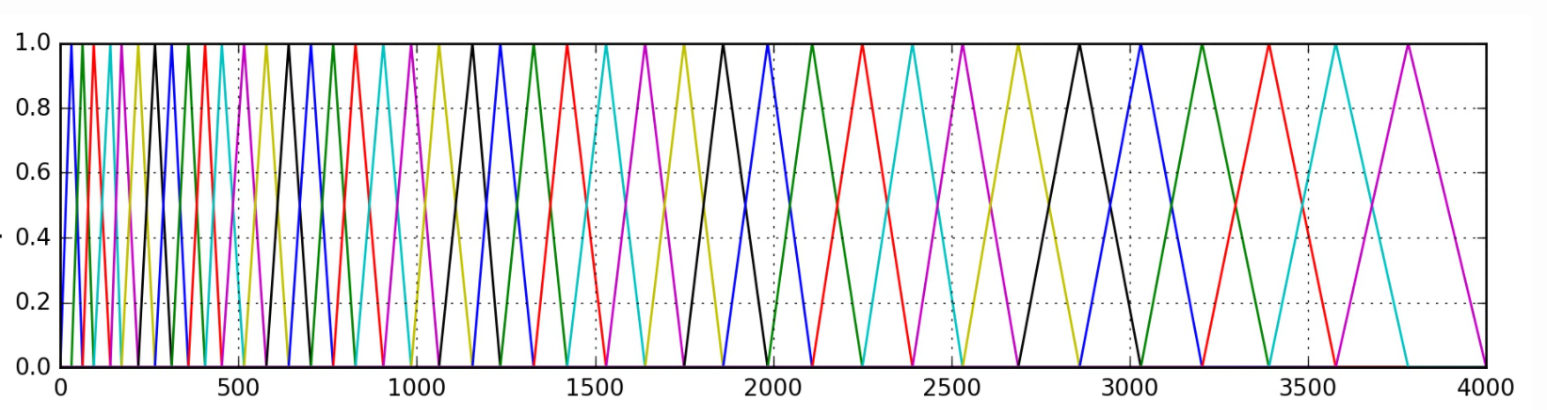
\includegraphics[width = 0.7\textwidth]{figures_ning/audio_5.png}
	\caption[Filter bank on a Mel-scale]
	{ Filter bank on a Mel-scale}
	\label{fig:audio_5}
\end{figure}

\subsection{Mel-spectogram Feature}

In machine learning, each audio segment can be represented by a corresponding mel-spectogram, and each frame corresponding to a certain frequency band is a feature. In practice, each audio has to be of the same length so that we have the same number of features. Usually, normalization is also performed, i.e., each element of each frame is subtracted from the average value of that frame to ensure that the average value of each frame is 0. Finally, the Mel-spectrogram is obtained as follows:

\begin{figure}[!htbp]
	\centering
	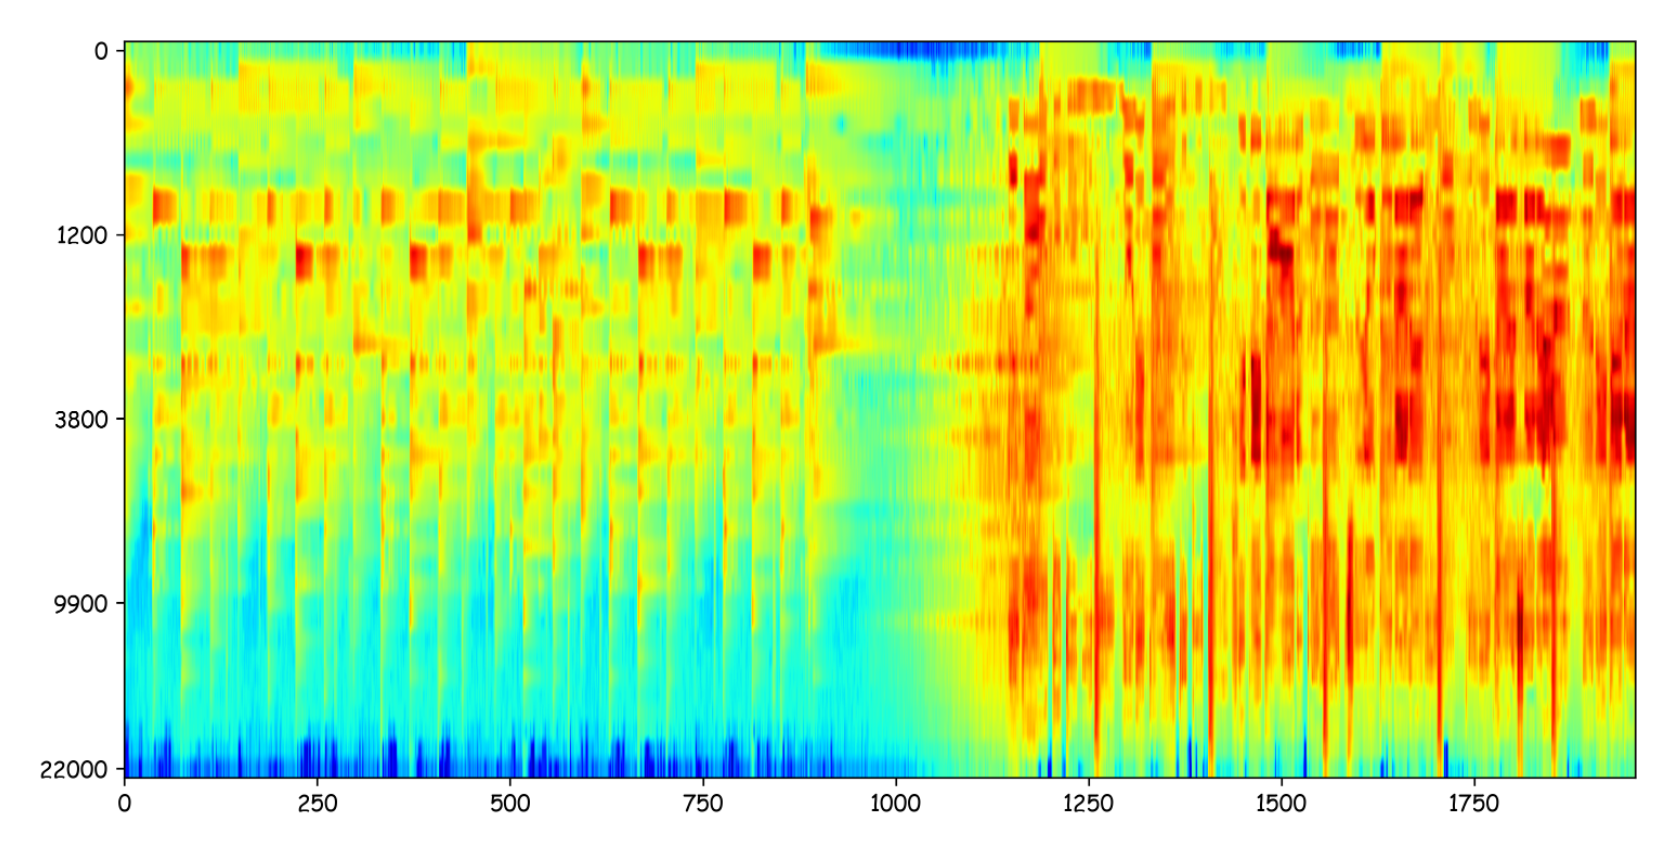
\includegraphics[width = 0.7\textwidth]{figures_ning/audio_6.png}
	\caption[Mel-spectogram]
	{ Mel-spectogram}
	\label{fig:audio_6}
\end{figure}

\subsection{VGG16}

VGG16 is a convolutional neural network model proposed by K. Simonyan and A. Zisserman from the University of Oxford in the paper ``Very Deep Convolutional Networks for Large-Scale Image Recognition''~\cite{simonyan2015deep}. The model achieves 92.7\% top-5 test accuracy in ImageNet~\cite{ILSVRC15}, which is a dataset of over 14 million images belonging to 1000 classes.

The structure of VGG16 is shown in Fig.~\ref{fig:vgg16}.The input to cov1 layer is of fixed size 224 x 224 RGB image. The image is passed through a stack of convolutional (conv.) layers, where the filters were used with a very small receptive field: 3x3 (which is the smallest size to capture the notion of left/right, up/down, center). In one of the configurations, it also utilizes 1x1 convolution filters, which can be seen as a linear transformation of the input channels (followed by non-linearity). The convolution stride is fixed to 1 pixel; the spatial padding of conv. layer input is such that the spatial resolution is preserved after convolution, i.e. the padding is 1-pixel for 3x3 conv. layers. Spatial pooling is carried out by five max-pooling layers, which follow some of the conv.  layers (not all the conv. layers are followed by max-pooling). Max-pooling is performed over a 2x2 pixel window, with stride 2.

Three Fully-Connected (FC) layers follow a stack of convolutional layers (which has a different depth in different architectures): the first two have 4096 channels each, the third performs 1000-way ILSVRC classification and thus contains 1000 channels (one for each class). The final layer is the soft-max layer. The configuration of the fully connected layers is the same in all networks.

All hidden layers are equipped with the rectification (ReLU) non-linearity. It is also noted that none of the networks (except for one) contain Local Response Normalisation (LRN), such normalization does not improve the performance on the ILSVRC dataset, but leads to increased memory consumption and computation time.


\begin{figure}[!htbp]
	\centering
	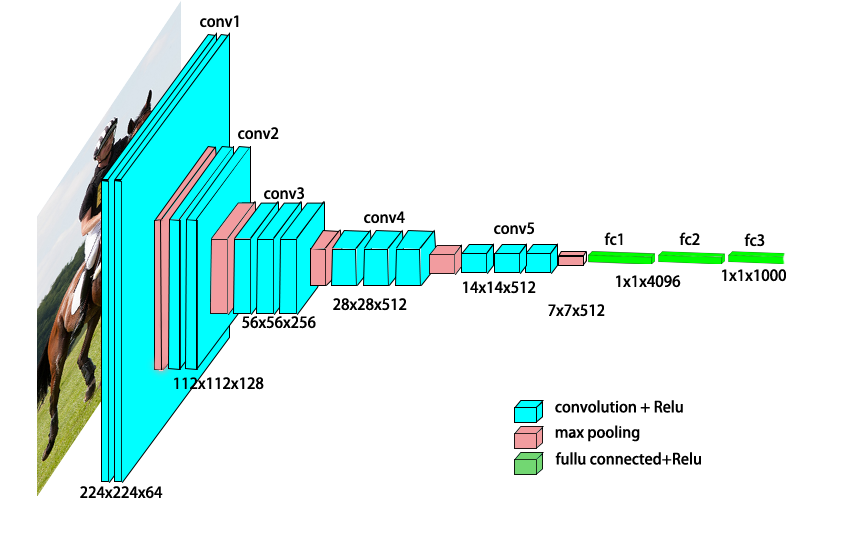
\includegraphics[width=0.8\linewidth]{figures/vgg16}
	\caption[The Architecture of VGG-16]{The Architecture of VGG-16.}
	\label{fig:vgg16}
\end{figure}

The advantages of VGG:
\begin{itemize}
	\item The structure of VGGNet is very simple, the entire network uses the same size of the convolution kernel size (3x3) and maximum pooling size (2x2).
	\item The combination of several small filter (3x3) convolutional layers is better than a large filter (5x5 or 7x7) convolutional layer.
	\item It is verified that performance can be improved by continuously deepening the network structure.
\end{itemize}

The disadvantages of VGG:

\begin{itemize}
	\item VGG consumes more computing resources and uses more parameters, resulting in more memory usage. Most of the parameters are from the first fully connected layer. VGG has 3 fully connected layers.
\end{itemize}



